\newcommand{\primalDescription}{
\section{Primal}
\epigraph{\textit{
    "A spirit took me in, when neither of my parents would
    accept me. Athas provides for those who care for it. We
    live in a desert simply because no-one cares for the land."
} }{
    Sutura, half‐elven druid
}
    Athasian primal casters, often refered to as druids,
    are the protectors of Athas' dying
    landscape. Patient and often unforgiving, they try to
    preserve and reclaim the barren lands that surround the
    Tyr region. Well armed with spells and abilities from the
    Spirits of the Land, they work to bolster Athas’ failing
    ecology.
    Often, druids prefer to remain hidden, observing the
    behavior of creatures and people before passing
    judgment. Travelers to an oasis are often unaware they
    are being observed; wanton destruction of the oasis will
    find themselves under the full fury of the druid and his
    many abilities.
    \\
    See \nref{tlttree:primal} for more information.
}

\newcommand{\primalTree}{
    \newpage
    \subsection{Primal Talent Tree}
    \label{tlttree:primal}

    \textbf{Class Skills:} Alchemy, Knowledge (Nature), Primal (Augment), Primal (Conjure), Primal (Curse), Primal (Shape)
    \newline

    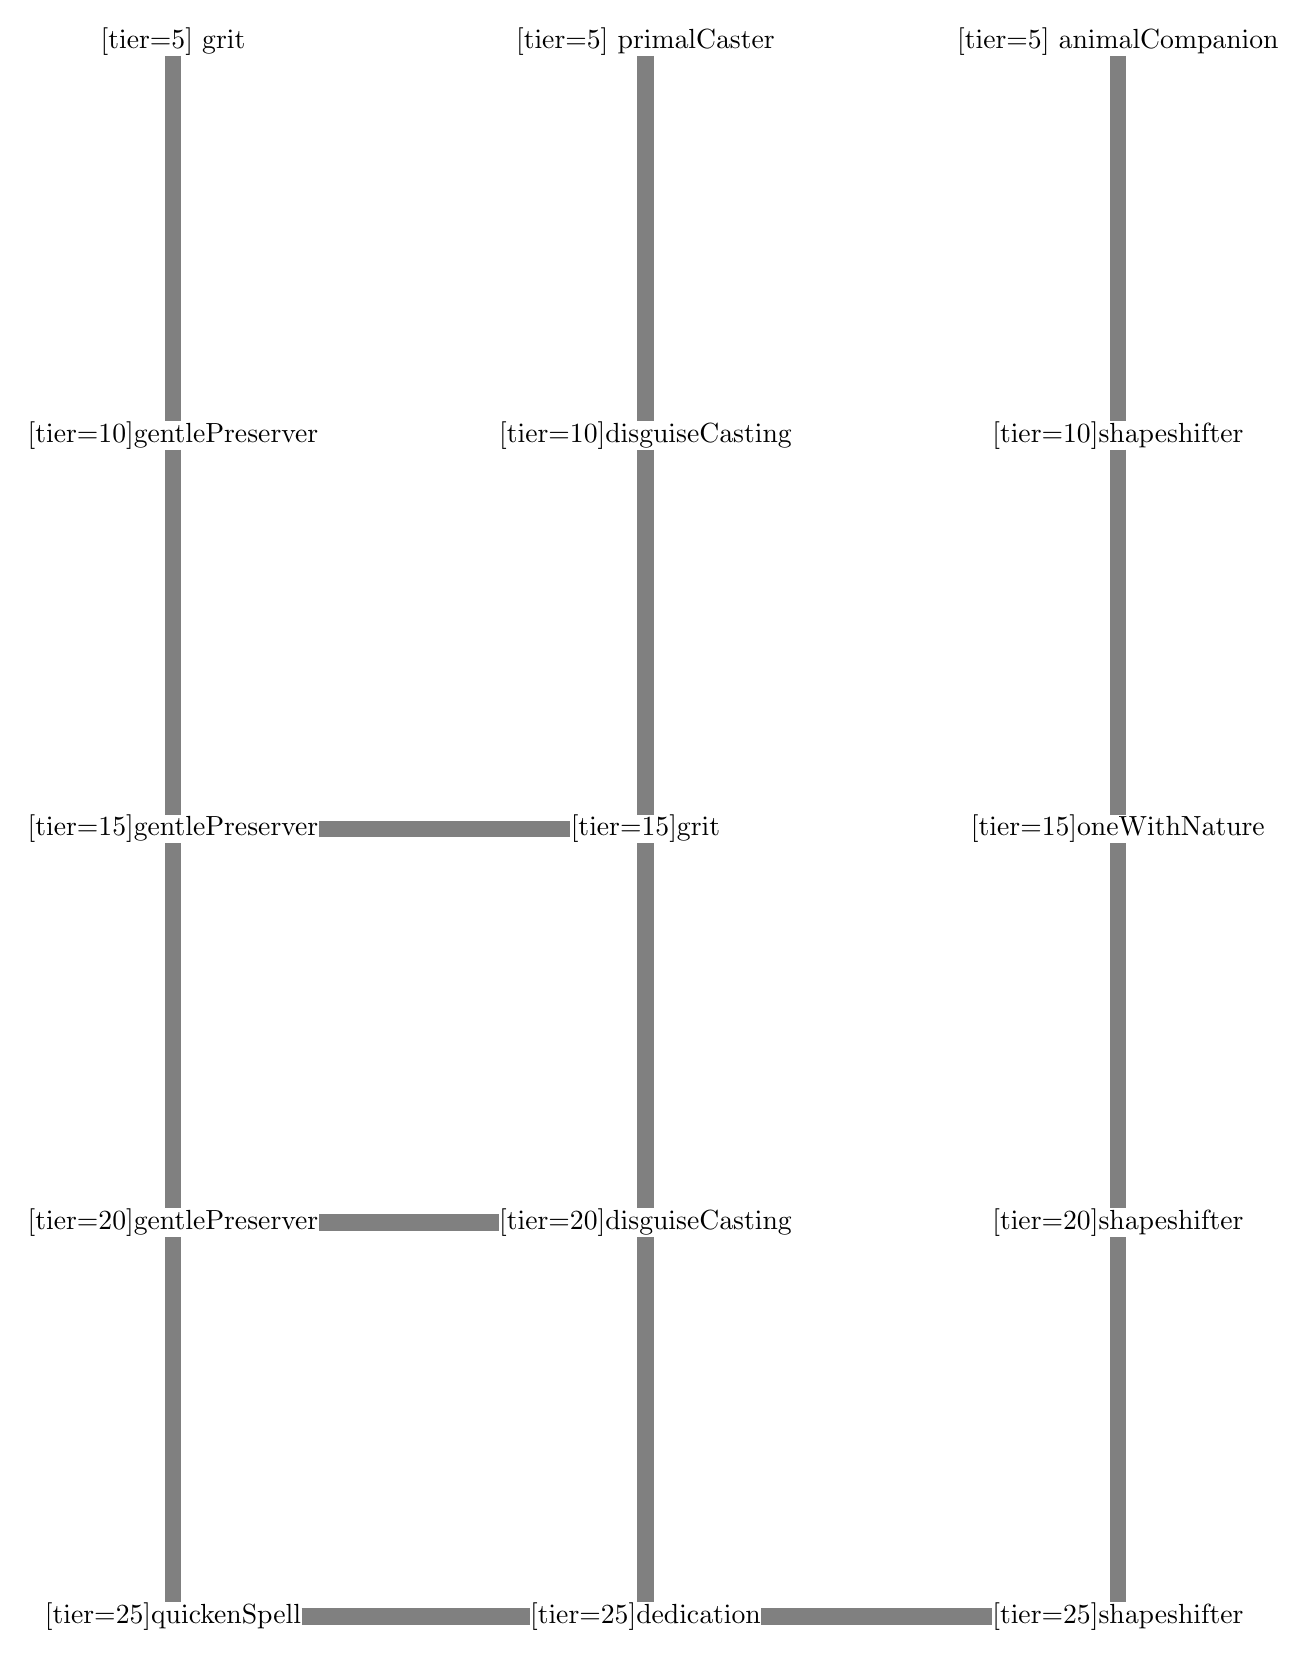
\begin{tikzpicture}
        \draw ( 0,  0) node(aa)[inner sep=0]{\TalentBox[tier=5] {grit}}
              ( 6,  0) node(ab)[inner sep=0]{\TalentBox[tier=5] {primalCaster}}
              (12,  0) node(ac)[inner sep=0]{\TalentBox[tier=5] {animalCompanion}}
              ( 0, -5) node(ba)[inner sep=0]{\TalentBox[tier=10]{gentlePreserver}}
              ( 6, -5) node(bb)[inner sep=0]{\TalentBox[tier=10]{disguiseCasting}}
              (12, -5) node(bc)[inner sep=0]{\TalentBox[tier=10]{shapeshifter}}
              ( 0,-10) node(ca)[inner sep=0]{\TalentBox[tier=15]{gentlePreserver}}
              ( 6,-10) node(cb)[inner sep=0]{\TalentBox[tier=15]{grit}}
              (12,-10) node(cc)[inner sep=0]{\TalentBox[tier=15]{oneWithNature}}
              ( 0,-15) node(da)[inner sep=0]{\TalentBox[tier=20]{gentlePreserver}}
              ( 6,-15) node(db)[inner sep=0]{\TalentBox[tier=20]{disguiseCasting}}
              (12,-15) node(dc)[inner sep=0]{\TalentBox[tier=20]{shapeshifter}}
              ( 0,-20) node(ea)[inner sep=0]{\TalentBox[tier=25]{quickenSpell}}
              ( 6,-20) node(eb)[inner sep=0]{\TalentBox[tier=25]{dedication}}
              (12,-20) node(ec)[inner sep=0]{\TalentBox[tier=25]{shapeshifter}}
        ;

        \tikzstyle{bar}=[gray,-,>=stealth, line width=6pt]

        \draw [bar] (aa) to (ba);
        \draw [bar] (ab) to (bb);
        \draw [bar] (ac) to (bc);

        \draw [bar] (ba) to (ca);
        \draw [bar] (bb) to (cb);
        \draw [bar] (bc) to (cc);

        \draw [bar] (ca) to (da);
        \draw [bar] (cb) to (db);
        \draw [bar] (cc) to (dc);

        \draw [bar] (da) to (ea);
        \draw [bar] (db) to (eb);
        \draw [bar] (dc) to (ec);

        \draw [bar] (ca) to (cb);

        \draw [bar] (da) to (db);

        \draw [bar] (ea) to (eb);
        \draw [bar] (ec) to (eb);
    \end{tikzpicture}
}
